\documentclass{beamer}
\usepackage[utf8]{inputenc}
\usepackage{amsmath}
\usepackage{amsfonts}
\usetheme{Madrid}
\usecolortheme{beaver}

\title{Cyclic Redundancy Check - 8}
\subtitle{ACA}
\author{André Alves 88811 \\ \and Renato Valente 89077}
\date{December 2020}
\institute[UA]{Departamento de Eletrónica, Telecomunicações e Informática\\Universidade de Aveiro}

\begin{document}
\maketitle

% \begin{frame}
% \frametitle{Introduction}
% \textbf{CRC  (Cyclic Redundancy Check)} é um algoritmo de verificação para detectar inconsistência de dados, como por exemplo erros de bit durante a transmissão de dados. \\
% CRC usa um Gerador Polinomial em que o polinómio b(x) é chamado de polinómio gerador para um esquema CRC cujo número de bits é definido pelo grau de b(x). Uma possível escolha para strings de até 64 bits é \textbf{CRC-8 AutoSar}, onde o polinómio gerador é: $ x^8 + x^5 + x^3 + x^2 + x + 1 $
% Este polinómio representa a chave binária: \textbf{100101111}

% $$ ( \sum_{n=0}^{15} a_{n} \times x^{n+8} ) mod ( x^8 + x^5 + x^3 + x^2 + x + 1 ) $$


% \end{frame}

\begin{frame}
\frametitle{Encoder}

    Para a codificação dos dados usamos as Propriedades do módulo (Properties of the remainder).\\
    $$ ( \sum_{n=0}^{15} a_{n} \times x^{n+8} ) mod ( x^8 + x^5 + x^3 + x^2 + x + 1 ) $$ 
    Com a resolução da fórmula anterior podemos concluir que são necessários \textbf{64 xor} gates e \textbf{11 xor} de atraso de propagação no pior caso.\\
    Para reduzir o número de gates recorremos à utilização de operações comuns com execução em paralelo para a redução do atraso de propagação. \\
    Obtivemos uma redução na implementação para \textbf{38 XOR}-gates e \textbf{4 XOR}-gates de atraso de propagação no pior caso.\\
    A maneira como reduzimos as XOR-gates e a arquitetura do encoder encontram-se nos slides seguintes.

\end{frame}

\begin{frame}
\frametitle{Tabela de XOR-gates}
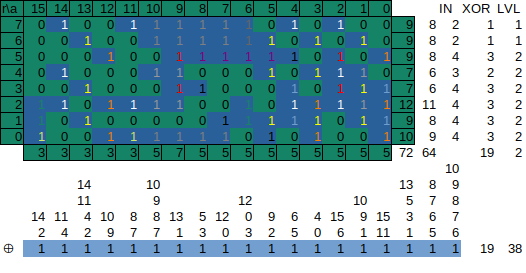
\includegraphics[scale=0.55]{tabela.png}\\
    As cores iguais equivalem à junção dessas entradas para poderem ser reaproveitadas ou para diminuir o atraso. Agrupámos 19 vezes as várias entradas, dando por isso, 19 XOR-gates.
    O Encoder agora com menos entradas precisa apenas de 19 XOR-gates, dando um total de 38 XOR-gates.
\end{frame}

\begin{frame}
\frametitle{Arquitetura}
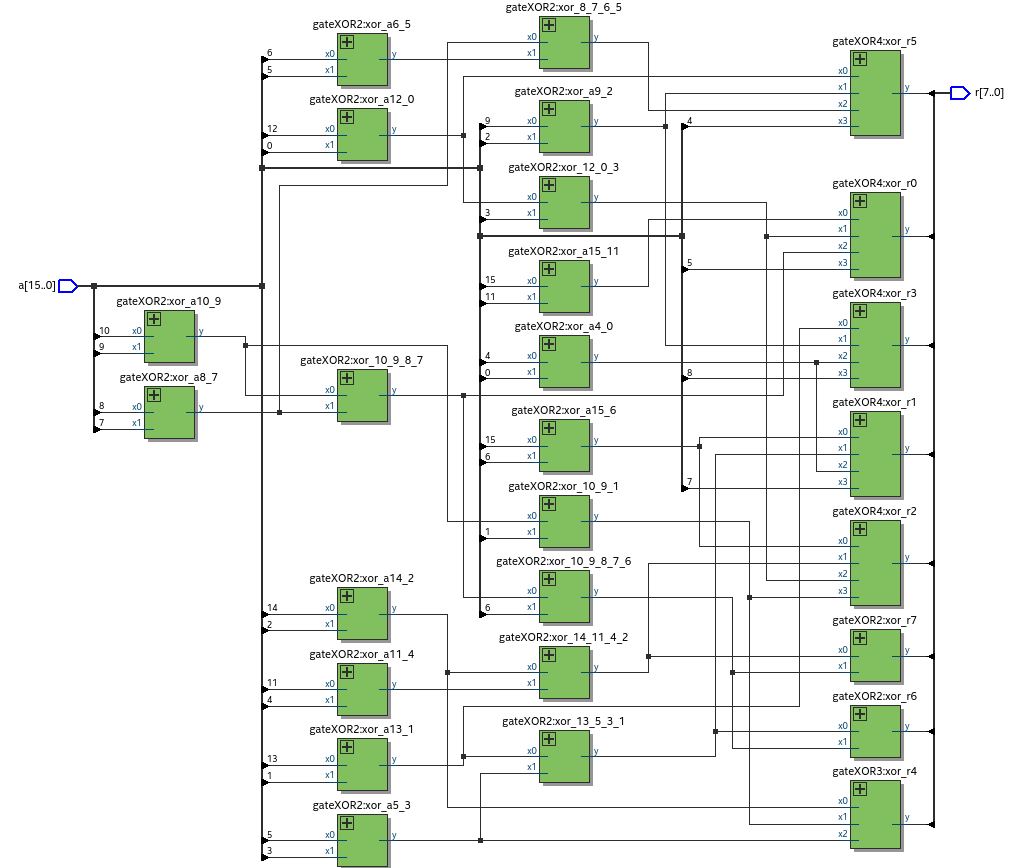
\includegraphics[scale=0.25]{arq.png}
\end{frame}

\begin{frame}
\frametitle{Arquitetura Extenso}
    Igual à anterior mas passando as gates XOR-4 para gates XOR-2.
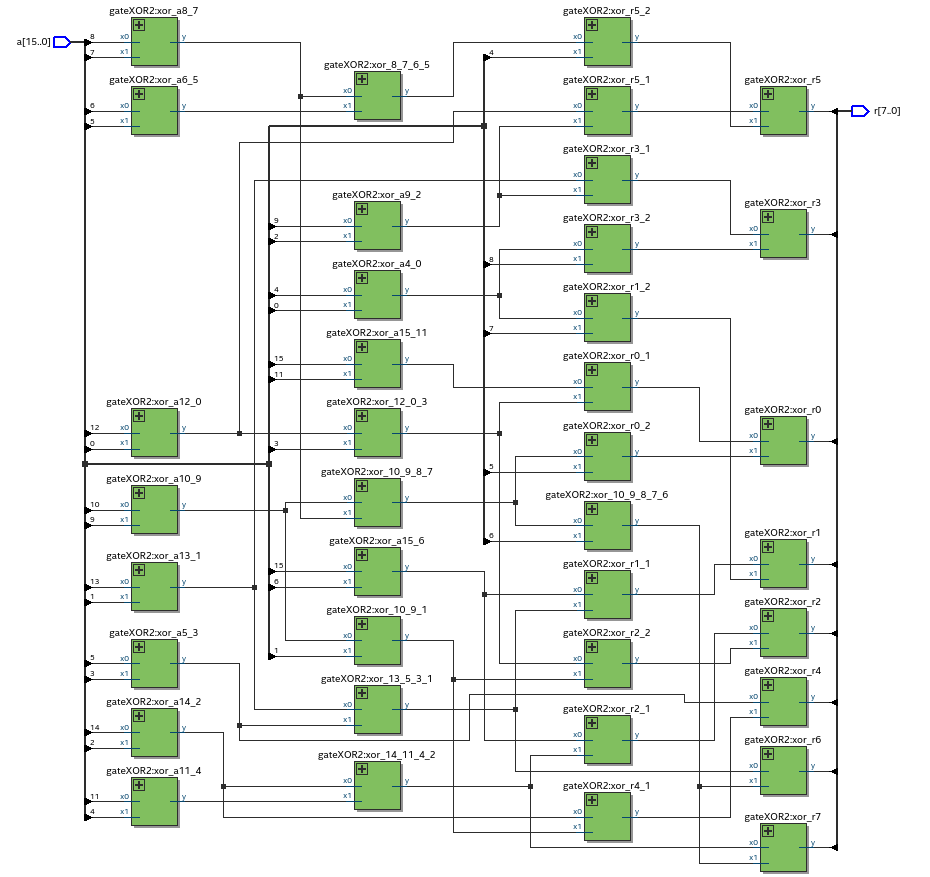
\includegraphics[scale=0.245]{arq_extenso.png}
\end{frame}

\begin{frame}
\frametitle{Checker}
    Verificar se existem erros introduzidos na transmissão.\\
    Para isso aceitamos a entrada de $\boldsymbol{a(x) \times x^8 + r}$ (a\_r), em que o $\boldsymbol{a(x)}$ é a nossa word em bits e o r é o resto da divisão do $\boldsymbol{a(x)}$ pelo polinómio $\boldsymbol{b(x)}$.\\
    Usamos os 16 primeiros bits da entrada ,\textbf{a\_r} na entrada \textbf{a} do encoder e recebemos o \textbf{r}. Depois fazemos comparação bit a bit do \textbf{r} dado pelo encoder com os 8 bits menos significativos da entrada \textbf{a\_r} usando XOR-gates de 2 entradas. Para não dar erro é necessário que todos os bits de comparação sejam 0, por isso usamos um OR-gate de 8 entradas, em que os bits de comparação são as entradas e a saída é a saída do checker. Saíndo 0 significa que a mensagem não contém erros.\\
    Esquema da arquitetura no slide seguinte.
    % Inicialmente separamos o $\boldsymbol{a(x)}$ do r e calculamos com o Encoder o $\boldsymbol{a(x)}$ obtendo assim o resto da divisão. Se esse resto da divisão for igual ao r quer dizer que a mensagem não contem erros.
\end{frame}

\begin{frame}
\frametitle{Arquitetura Checker}
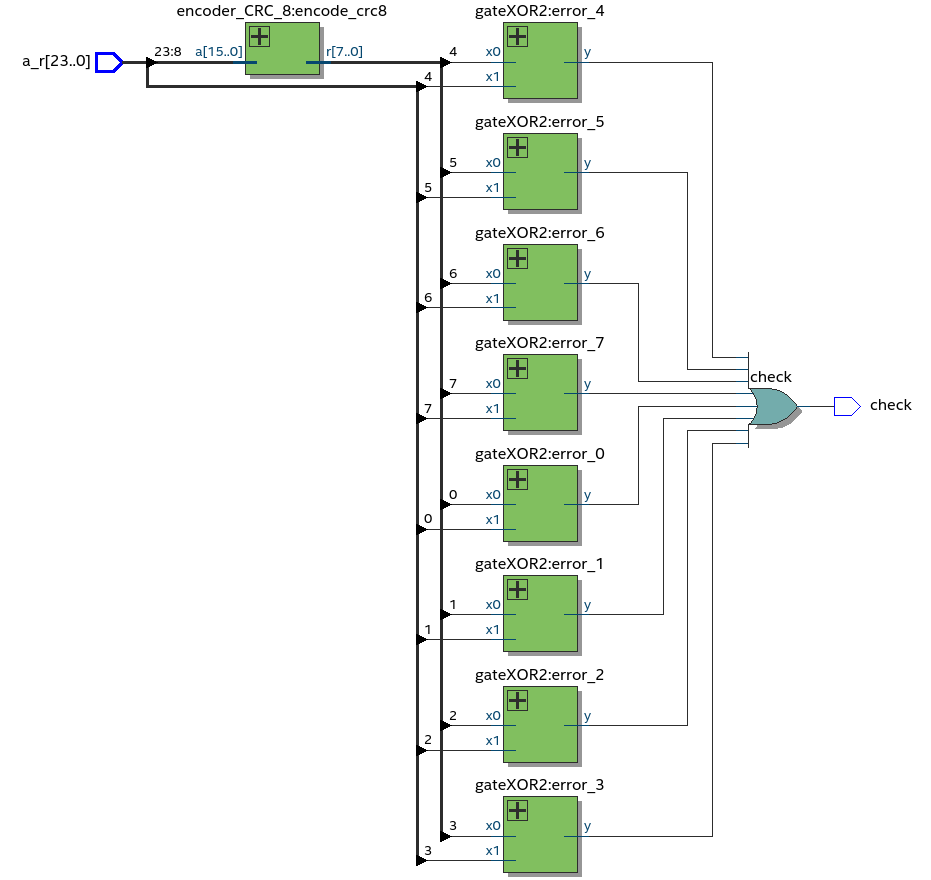
\includegraphics[scale=0.25]{arq_checker.png}
\end{frame}


\end{document}
